\documentclass[11pt]{article}
\usepackage[T1]{fontenc}
\usepackage{lmodern}
\usepackage[margin=1in]{geometry}
\usepackage{amsmath,amssymb,amsthm,mathtools}
\usepackage{booktabs,longtable,tabularx,array}
\usepackage{enumitem,microtype,xcolor,xurl}
\usepackage{tikz}
\usepackage{hyperref,fancyhdr,listings}
\hypersetup{colorlinks=true,linkcolor=blue!45!black,citecolor=blue!45!black,urlcolor=blue!50!black,pdftitle={Affine-plane contraction plans for exact SAT},pdfauthor={Research prepared for Vladimir Reshetnikov with ChatGPT}}
\setlength{\headheight}{14pt}
\pagestyle{fancy}\fancyhf{}
\fancyhead[L]{\small Affine-plane contraction plans}
\fancyhead[R]{\small Research iteration, 26 October 2026}
\fancyfoot[C]{\thepage}
\setlist{itemsep=3pt,topsep=5pt}
\newtheorem{theorem}{Theorem}[section]
\newtheorem{lemma}[theorem]{Lemma}
\newtheorem{proposition}[theorem]{Proposition}
\newtheorem{corollary}[theorem]{Corollary}
\theoremstyle{definition}\newtheorem{definition}[theorem]{Definition}
\theoremstyle{remark}\newtheorem{remark}[theorem]{Remark}
\newcommand{\poly}{\operatorname{poly}}
\newcommand{\F}{\mathbb F}
\newcommand{\K}{\mathcal K}
\newcommand{\pc}{\operatorname{popcount}}
\newcommand{\norm}[1]{\left\lVert#1\right\rVert_2}
\newcommand{\ceil}[1]{\left\lceil#1\right\rceil}
\newcommand{\floor}[1]{\left\lfloor#1\right\rfloor}
\newcommand{\CT}{30.2570356114963815\ldots}
\newcommand{\CS}{25.9890677186902171\ldots}
\lstset{basicstyle=\ttfamily\small,breaklines=true,frame=single,columns=fullflexible,keepspaces=true}
\title{\textbf{Affine-Plane Contraction Plans}\\[4pt]
\large Smaller Exponent Coefficients and a Joint Time--Space Certificate\\
for the Exact SAT Contraction Framework}
\author{Research prepared for Vladimir Reshetnikov with ChatGPT}
\date{26 October 2026 (Pacific time)}
\begin{document}
\maketitle
\begin{abstract}
We review twenty placed refinement packets and nine newer incoming packets in
ProveIt's SubexponentialSAT project, and incorporate the newly public Anthropic
formalization identified during this session. A new four-plan construction
from the affine plane $\F_3^2$ improves the cached contraction bound. On the
same generic normalized interface as the preceding coefficient comparisons,
with $s$ Boolean wires, the resulting deterministic algorithm has
\begin{align*}
 T&\le\poly(s+\mathcal L)\,2^{(\CT+o(1))s/\sqrt{\ceil{\log_2s}}},\\
 S&\le\poly(s+\mathcal L)\,2^{(\CS+o(1))s/\sqrt{\ceil{\log_2s}}}.
\end{align*}
The preceding best explicit comparable cached certificate was
$30.891018920366\ldots$ time and $30.753912832055\ldots$ space.
The improvement is a smaller leading coefficient in an exponential upper
bound; it does not change the general SAT exponent's logarithmic order.
The main new ingredient is an exact joint selector controlling both the
matrix-operation supports and the actual table boundaries. A rational
$9\to12\to9\to7\to4$ schedule pays for recursive entry evaluations.
The package supplies the proof, exact integer and rational checks, an exact
selector, and finite contraction tests. It does not contain an end-to-end
fast SAT solver or a new Lean formalization. The underlying deformation,
packing, recovery, and SAT reductions remain explicit imported dependencies.
\end{abstract}
\clearpage
\tableofcontents
\newpage

\section{Outcome, comparison, and scope}
\label{sec:outcome}

Let $E(s)=s/\sqrt{\ceil{\log_2s}}$. The size $s$ is the normalized Boolean
wire budget of the contraction theorem, not the SAT variable count $n$.
Initial precision and coefficient truncation are at most $s$, maximum root
degree is at most $\ceil{s^{9/10}}$, and the admissible entry-access conventions
are those specified in Section~\ref{sec:interface}. Under these common
premises our main result is
\begin{equation}\label{eq:main}
 T\le\poly(s+\mathcal L)2^{(C_T+o(1))E(s)},\qquad
 S\le\poly(s+\mathcal L)2^{(C_S+o(1))E(s)},
\end{equation}
where
\begin{align}
 \kappa&=\frac{\pi\sqrt2}{\ln2},\notag\\
 C_T&=\kappa\left[
  \frac49\sqrt{\frac{100000}{1577}}
  +\frac{\sqrt{137}}{90}\sqrt{\frac{25000}{303}}\right]
  =\CT,\label{eq:timeconstant}\\
 C_S&=\kappa\sqrt{\frac7{27}}\sqrt{\frac{100000}{1577}}
  =\CS.\label{eq:spaceconstant}
\end{align}
Thus $30.26$ and $26.00$ are safe eventual time and space coefficients.

\begin{center}
\begin{tabular}{>{\raggedright\arraybackslash}p{6.5cm}rr}
\toprule
Comparable generic certificate & Time & Space\\\midrule
Best placed cached packet, \emph{subsat\_contraction\_tree}
 &35.354588&34.274803\\
Newest incoming best, \emph{sat\_adaptive\_tree\_certificate}
 &30.891019&30.753913\\
This report, same $12/5$ matrix exponent allowance
 &\textbf{30.257036}&\textbf{25.989068}\\\bottomrule
\end{tabular}
\end{center}
The numerical reductions against the incoming best are approximately
$2.0523\%$ in the time coefficient and $15.4935\%$ in the space coefficient.
They are not measured runtime or memory ratios. For example, the ratio of
the two displayed leading time-bound functions is
$2^{-(0.6339833088\ldots)E(s)}$; actual algorithms may run much faster than
their upper bounds, and finite-size overheads are substantial.

The strongest inspected polynomial-space certificate is still
$46.184845586731\ldots$, from the incoming adaptive-flags packet
\cite{flags}. This report does not improve that resource regime. Keeping
that algorithm and the stronger-assumption low-degree branches available
preserves their guarantees. The independent Anthropic theorem has an
unspecified absolute constant, so its running time cannot be numerically
ranked against these wire-normalized coefficients.

\paragraph{What is new.}
The four directions in $\F_3^2$ give four mutually orthogonal ways to
partition nine groups into three triples. Their matrix-operation supports
have exact cross inner products small enough to improve the uniform
adaptive bound. Tracking table-boundary supports at the same time gives
a stronger memory theorem without increasing the time coefficient.
The supplied selector makes this joint choice using integers. The
support-averaging principle, matrix multiplication, and basic affine-plane
geometry are established tools; the new contribution is their specific
combination and quantitative certificate relative to the reviewed corpus.
We do not claim literature-wide priority or global optimality.

\paragraph{What remains open.}
For fixed clause width, the inherited general SAT order remains
\begin{equation}\label{eq:satorder}
 (n+m)^{O_k(1)}2^{O_k(n\log\log n/\sqrt{\log n})}.
\end{equation}
The fixed-density order remains $2^{O_{k,D}(n/\sqrt{\log n})}$.
No proof of a smaller logarithmic order emerged from this iteration.
The conditional $n\log\log n/\log n$ proposals still lack their stated
summation or representation interface. This distinction is essential to
interpreting the improvement in \eqref{eq:main}.

\section{Frozen review and the new Anthropic source}
\label{sec:review}

\subsection{Repository scope}
The ProveIt checkout is pinned at
\path{73dfb5e5ab6e91bd7375e5b97ef85d7e1cc8e81d}.
The relevant placement commits are \texttt{2b925d8800},
\texttt{6d3adc4506}, and \texttt{450252e9d8}; the nine newer incoming ZIPs
were committed by \texttt{b9941a7396}. Both requested directories were
inspected. Twenty placed packets and all nine incoming packets were screened
for headline theorems and scope. Detailed proof review concentrated on the
strongest generic cached and polynomial-space certificates and the
interfaces used below. This is not an independent verification of every
claim in all twenty-nine packets.

The original project summary still names $55.70948$ as the smallest
polynomial-space coefficient and $35.35459$ as the smallest cached time
coefficient. The newer incoming files supersede those comparison numbers.
Table~\ref{tab:incoming} records their generic claims, suppressing polynomial
factors and the common $E(s)$ scale. A dash means that the packet does not
provide a new coefficient in that column. The full source inventory and
hashes are supplied separately.

\begin{table}[ht]
\centering\small
\begin{tabular}{p{6.3cm}rrr}
\toprule Incoming packet & PS time & Cached time & Cached space\\\midrule
\path{3sat_round3_frontier} &63.75736&37.93011&33.62304\\
\path{ETH_Adaptive_Exact_Kernels} &55.33163&35.07061&33.99950\\
\path{eth_adaptive_schedules} &63.78117&37.59170&33.62304\\
\path{sat_adaptive_bounds} &\textbf{46.18485}&34.32528&34.02418\\
\path{sat_adaptive_frontier} &50.30469&31.25240&31.25240\\
\path{sat_adaptive_matrix_partition} &50.21043&34.32528&34.02418\\
\path{sat_adaptive_tree_certificate} &---&\textbf{30.89102}&30.75391\\
\path{subexponential_sat_adaptive_four} &50.39373&32.91581&31.66171\\
\path{subsat_rectangular} &53.97753&33.99389&33.99372\\\bottomrule
\end{tabular}
\caption{Incoming claims at the frozen snapshot, using the packets' displayed
generic assumptions. The four-block packet also offers a different matrix
backend; that optional point does not beat the highlighted incoming time.}
\label{tab:incoming}
\end{table}

The strongest density-sensitive order retained in the portfolio is
\begin{equation}\label{eq:density}
 (n+m)^{O_k(1)}2^{O_k\left(
 \frac n{\sqrt{\log n}}
 \min\{\log(2+m/n),\log\log n\}\right)},
\end{equation}
in the parameter ranges established by the two density packets
\cite{density}. This improves some growing-density regimes, not the
unrestricted worst-case order. All comparisons with \eqref{eq:density}
keep its hypotheses and normalization separate from \eqref{eq:main}.

\subsection{Publication update supplied during the session}
The user supplied Anthropic pull request 31 at exact revision
\path{1a6eee293b9e00cb432eef6018a21f523623a9af} \cite{anthropic}.
It was merged on 26 October 2026 at 8:07:22 p.m. Pacific time. This changes
an outdated statement in the earlier ProveIt reports: the Claude paper's
Lean development is now publicly available.

The published \path{eth/MainResults.lean} defines one finite-alphabet
deterministic Mathlib TM2 machine and one constant $C$, both chosen before
$k$, with counting time
\begin{equation}\label{eq:anthropic}
 2^{C\min\{km/\sqrt{\log_2m},\;
 k^2n\log_2\log_2n/\sqrt{\log_2n}\}}.
\end{equation}
Its explicit premises are $k\ge1$, $m\ge2$, $n\ge4$, no repeated clause
lists, and occurrence of every named variable. The source also gives a
separate ETH-negation statement. \path{Solution.lean} contains proof terms
for both. \path{Challenge.lean} contains the intentional comparison stubs;
those stubs are not the proof terms in \path{Solution.lean}.

The README pins Lean and Mathlib v4.33.1 and gives build, axiom-inspection,
Comparator, and independent-kernel instructions. We inspected the statements,
entry points, paper, and source index; we did not rebuild the Lean development.
Accordingly this report attributes the formal verification claims to the
published project and does not report a new local proof-assistant check.
The new 49-page PDF differs in bytes from the older 49-page ProveIt copy;
its SHA-256 and the comparison are recorded in the package. Its headline
order is still \eqref{eq:anthropic}.

The Anthropic construction offers a distinct research interface, based on
integral decompositions of rectangle swaps and choosing a cheaper row or
column contraction. Section~\ref{sec:frontier} discusses its implication
for the next order-improvement attempt. It is not used as an unproved
shortcut in our new coefficient theorem.

\section{The normalized contraction interface}
\label{sec:interface}

We import the exact arithmetic and reduction framework of the OpenAI
manuscript and the compatible refinements \cite{openai,asymmetric,joint,trees}.
The root has at most $s$ wires and entries in
\[
 (\mathbb Z/2^{P_0}\mathbb Z)[V]/(V^\ell),\qquad P_0,\ell\le s,
\]
maximum degree at most $\ceil{s^{9/10}}$, and total description length
$\mathcal L$. Admissible original entry routines use polynomial space and
$\poly(s+\mathcal L)2^{O(s^{9/10})}$ time with fixed constants. The extension
ring, canonical lifts, and immutable creation-precision tags are retained.
In particular, a recursively created tensor is evaluated from its fixed
creation-time representatives, rather than by recursively rerunning its
whole ancestor contraction.

At an active call let $M$ be the current wire count, $r$ the fixed number
of groups, $u$ the retained interpolation range, $a$ the cumulative packet
exponent, and $D=2^{a-i}$ at retained valuation $i<u$. The inherited
mechanisms give near-unit padding, child size
$(2/r+o(1))M$, working precision $(6+o(1))MD/u$, and full-Cauchy modes with
weights
\[
 a+1-i+4q-2\pc(q),\qquad q\ge0.
\]
There are at most $(2+o(1))M/(r^2D)$ families per directed group pair and
index. These are mathematical dependencies, not newly proved facts here.

For each directed pair $g\ne h$, allocate an exact nonnegative mode weight
$b_{gh}$, with total below the working precision. Let $\mathcal I_{gh}$ be
the corresponding finite list. An empty list makes that allocation zero;
otherwise write $h_{gh}=\log_2|\mathcal I_{gh}|$. Its contribution is the
finite graphical sum
\begin{equation}\label{eq:graphsum}
 \sum_{\xi_{gh}\in\mathcal I_{gh}}
 \prod_{g=1}^r Z_g\bigl((\xi_e)_{e\ni g}\bigr),
\end{equation}
where evaluating an entry of $Z_g$ requires a real recursive contraction.
Exact list cardinalities and indexing are obtained by the ordinary
unbounded-knapsack recurrence. As $r$ ranges over a fixed finite set, the
number of exact-weight allocations is polynomial in $s$.

\begin{lemma}[Imported uniform entropy estimate]\label{lem:entropy}
Put $\K(M,u)=\kappa M/\sqrt u$, with $\kappa=\pi\sqrt2/\ln2$.
For every member of a fixed finite family of nonnegative directed weights
$z=(z_{gh})$,
\[
 \sum_{g\ne h}z_{gh}h_{gh}
 \le\left(\frac{\norm z}{r}+o(1)\right)\K(M,u).
\]
The error is uniform over the active depths and exact-weight allocations
of our schedule.
\end{lemma}
\begin{proof}[Source and normalization]
The full-Cauchy generating-function estimate is
\[
 \sum_{q\ge0}-\ln(1-e^{-\theta(1+4q-2\pc(q))})
 =\frac{\pi^2}{24\theta}+O(\log^2(2/\theta)).
\]
For pair $e$ use parameter $\theta/z_e$, multiply its logarithmic bound
by $z_e$, and sum. The leading expression is
$\theta p+\pi^2(2+o(1))M\sum_e z_e^2/(24\theta r^2D)$.
Using $p\le(6+o(1))MD/u$ and optimizing $\theta$ gives the displayed
constant after division by $\ln2$. The additive precision guard makes the
error lower order uniformly. This reproduces the normalization of the
inherited estimate; its mode factorization and precision premises are
imported from the cited packets.
\end{proof}

For an unordered pair $e=\{g,h\}$ define $g_e=h_{gh}+h_{hg}$. Thus for
any fixed nonnegative unordered support $w$,
\begin{equation}\label{eq:unordered}
 w\cdot g\le\left(\frac{\sqrt2\norm w}{r}+o(1)\right)\K(M,u).
\end{equation}
The factor $\sqrt2$ matters: a support on an undirected pair weights both
orientations in the underlying list representation.

\section{Operation and storage supports}
\label{sec:supports}

A plan partitions the groups into three nonempty ordered blocks. Within
each block it recursively splits an ordered list at its midpoint and
contracts the two resulting tables. It then contracts the final triangle
of three block tables. There are $r-3$ internal merges and one final
triangle. A subset table retains precisely the indices on its boundary.

For an internal merge, write the three disjoint vertex classes as $A,B,O$,
where $O$ is the complement of $A\cup B$. Let $H_1,H_2,H_3$ be the sums of
$g_e$ on its three crossing pair classes. With the same conservative
matrix exponent allowance $\omega<12/5$ used in the incoming best,
rectangular blocking gives operation time exponent
\begin{equation}\label{eq:mm}
 H_1+H_2+H_3-\frac35\min(H_1,H_2,H_3)
 =\max_j\left(\frac25H_j+\sum_{k\ne j}H_k\right).
\end{equation}
The final triangle has the same three forms. Multiplying by five gives
integer support vectors $v\in\{0,2,5\}^{\binom r2}$. For plan $j$, let
$\mathcal V_j$ be its $3(r-2)$ supports and put
\[
 F_j(g)=\frac15\max_{v\in\mathcal V_j}v\cdot g.
\]
For every table subset $S$ let $b_S$ be the $0$--$1$ indicator of its
unordered boundary. Include singleton input caches, internal subset tables,
and final block tables, and put
\[
 G_j(g)=\max_{S\text{ in plan }j}b_S\cdot g.
\]
The final product of two block tables has the boundary of the complementary
third block, so it is covered by the same list.

\begin{lemma}[Arithmetic and workspace]\label{lem:workspace}
After the singleton factor entries have been evaluated, a plan can be
executed with local time $\poly(s)2^{F_j(g)}$ and space
$\poly(s)2^{G_j(g)}$ over the inherited coefficient ring.
\end{lemma}
\begin{proof}
For matrix dimensions $a,b,c$, divide into square blocks of side
$m=\min(a,b,c)$. A fixed bilinear multiplication algorithm of exponent
below $12/5$ gives $abc\,m^{-3/5}$ work up to polynomial factors in record
length, yielding \eqref{eq:mm}. Such algorithms exist over characteristic
zero with a strict exponent margin \cite{mm}. The inherited coordinate/CRT
bridge expands each ring entry into polynomially many integer coordinates,
uses sufficiently many nonexceptional odd primes, reconstructs exact bounded
integer matrix products, applies the ring structure constants, and reduces
to the desired precision. It never divides by a nonunit of the original ring.
All coordinate counts and reconstruction bit lengths are polynomial in $s$.

Workspace deserves a separate argument. Implement the fixed bilinear
algorithm recursively, processing its fixed number of subproducts
sequentially and accumulating into the output. The work arrays at
successive sizes have a geometrically decreasing sum, so square
multiplication uses $O(m^2)$ scalar storage. Process rectangular blocks and
CRT coordinates sequentially. Storage is a polynomial factor times the
input and output matrix entries. Those matrices are exactly the subset
boundary tables counted by $G_j$, or submatrices of them. At most a constant
number of tables per plan coexist, since $r$ is fixed. This proves the
stronger boundary-based space bound; merely bounding storage by time
would lose the improvement below.
\end{proof}

The proof relies on the stated theoretical matrix backend. Our finite
contraction implementation uses ordinary exact scalar arithmetic to test
the regrouping, not an implementation of that asymptotic backend.

\section{Four plans from the affine plane}
\label{sec:affine}

Label the nine groups by $\F_3^2$, using labels $3x+y$ for
$x,y\in\{0,1,2\}$. The level sets of four projectively distinct nonzero
linear forms give four partitions into parallel lines. Use the following
ordered triples; their order also specifies the internal midpoint splits:
\begin{center}
\begin{tabular}{cl}
\toprule Plan & Three final blocks\\\midrule
0 & $(0,1,2)\mid(3,4,5)\mid(6,7,8)$\\
1 & $(0,3,6)\mid(1,4,7)\mid(2,5,8)$\\
2 & $(0,5,7)\mid(1,3,8)\mid(2,4,6)$\\
3 & $(0,4,8)\mid(2,3,7)\mid(1,5,6)$\\\bottomrule
\end{tabular}
\end{center}
Any line from one partition meets any line from another in one point.
Every unordered pair is internal to one of the four partitions and crosses
the other three. These two exact incidence properties drive the bound.

\begin{figure}[ht]
\centering
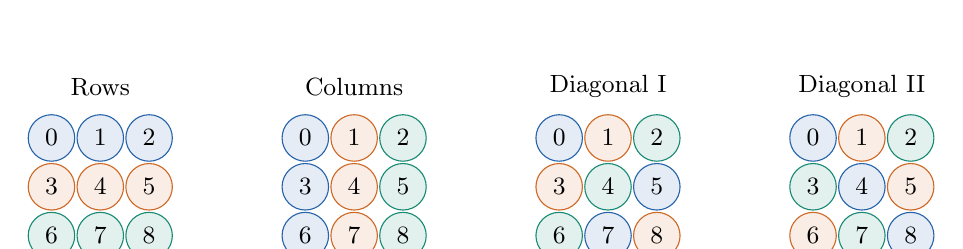
\begin{tikzpicture}[x=0.62cm,y=0.62cm]
\definecolor{classa}{RGB}{37,99,170}
\definecolor{classb}{RGB}{206,104,36}
\definecolor{classc}{RGB}{24,138,116}
\foreach \p/\title in {0/Rows,1/Columns,2/Diagonal I,3/Diagonal II}{
 \begin{scope}[shift={(5.2*\p,0)}]
 \node[font=\small] at (1,3.05) {\title};
 \foreach \x in {0,1,2}{\foreach \y in {0,1,2}{
  \pgfmathtruncatemacro{\idx}{3*\x+\y}
  \ifcase\p\pgfmathtruncatemacro{\cl}{\x}\or
  \pgfmathtruncatemacro{\cl}{\y}\or
  \pgfmathtruncatemacro{\cl}{mod(\x+\y,3)}\or
  \pgfmathtruncatemacro{\cl}{mod(\y-\x+3,3)}\fi
  \ifcase\cl\def\cc{classa}\or\def\cc{classb}\or\def\cc{classc}\fi
  \node[circle,draw=\cc,fill=\cc!12,minimum size=5.5mm,font=\small] at (\y,2-\x) {\idx};
 }}
 \end{scope}
}
\end{tikzpicture}
\caption{The same nine groups under four partitions. Each color class is one
three-group block; the diagram displays finite-field classes, not Euclidean
line segments.}
\end{figure}

Each plan has twenty-one operation supports and fifteen stored-table
boundary supports: nine singletons, three two-point subsets, and three
lines. We use both support families in the selector.

\begin{lemma}[Exact affine support bounds]\label{lem:affinebounds}
For a time support $t=v/5$ and a boundary support $b$ of any plan,
\[
 \norm t^2\le\frac{486}{25},\qquad \norm b^2\le18.
\]
For supports belonging to distinct affine directions,
\begin{equation}\label{eq:crossbounds}
 t\cdot t'\le\frac{288}{25},\qquad
 b\cdot b'\le8,\qquad t\cdot b'\le\frac{48}{5}.
\end{equation}
\end{lemma}
\begin{proof}
For a time operation the three class sizes are $(1,1,7)$, $(1,2,6)$, or
$(3,3,3)$. Its maximum integer squared norm is respectively $354$, $458$,
or $486$. This follows by assigning the discounted coefficient two to
the smallest crossing class and coefficient five to the other classes.

For two directions the $3\times3$ array of intersections has one point
per cell. Enumerating the three possible discounted pair classes in each
operation gives the following upper bounds on integer inner products:
\begin{center}
\begin{tabular}{c|rrr}
 & $(1,1,7)$ & $(1,2,6)$ & $(3,3,3)$\\\hline
$(1,1,7)$&204&208&215\\
$(1,2,6)$&208&240&260\\
$(3,3,3)$&215&260&288
\end{tabular}
\end{center}
These finite counts can be reconstructed directly by assigning each pair
of labels its operation classes. The independent verifier supplied with
this paper enumerates all $6\cdot21^2=2646$ cross-direction time pairs,
all self norms, and both mixed families, using only integer membership
tests. Thus the table is a complete finite certificate, not a sample.

There is also a useful direct explanation of the largest entry. A final
time support is the indicator of the twenty-seven crossing pairs minus
$3/5$ times the indicator of one discounted nine-pair class. Across two
directions, the full crossing sets meet in eighteen pairs, a discounted
class meets the other's full crossing set in six, and the two discounted
classes meet in two. Their inner product is therefore
$18-(3/5)12+(9/25)2=288/25$, independently of the chosen discounts.

For boundaries of subsets $S,T$ of sizes $a,b\le3$, contained in lines of
different directions, $c=|S\cap T|$ is zero or one. Their boundary
intersection has size
\[
 c(9-a-b+c)+(a-c)(b-c).
\]
If $c=1$, this is $(a-2)(b-2)+7\le8$. If $c=0$, it is $ab$; $a=b=3$
is impossible because the two full lines meet, so it is at most six.
Also $|\partial S|=a(9-a)\le18$.
Finally, enumerating the same $3\times3$ intersections for a time
operation and a boundary gives $48/5$. For a final time operation and a
line boundary this is $12-(3/5)4=48/5$; smaller subsets and internal
operations are no larger, as the complete finite check confirms.
\end{proof}

\begin{corollary}[Affine local time]\label{cor:affinetime}
Selecting the least-time affine plan gives local aggregation exponent
at most $(1/\sqrt3+o(1))\K(M,u)$.
\end{corollary}
\begin{proof}
Choose a maximizing support in each of the four plans. The squared norm
of their sum is at most
$4(486/25)+12(288/25)=216$.
The minimum of four maxima is at most their average. Apply
\eqref{eq:unordered} to the average support: its squared norm is at most
$216/16$, and $\sqrt{2(216/16)}/9=1/\sqrt3$.
Equality in the support-norm certificate is attained by any choice of four
final-triangle supports. This establishes the certificate value, not a
global algorithmic optimality claim.
\end{proof}

\section{A joint selector improves memory as well}
\label{sec:jointselector}

Minimizing time and minimizing storage independently would select
potentially different plans. It would not establish a simultaneous
time--space pair. The following selector resolves this issue explicitly.

\begin{theorem}[Joint affine time--space certificate]\label{thm:joint}
Set $\rho=3/\sqrt7$. Select a plan minimizing an upward-rounded proxy for
\[
 J_j(g)=\max\{F_j(g),\rho G_j(g)\}.
\]
Then, uniformly over the feasible mode allocations,
\[
 F_j(g)\le\left(\frac1{\sqrt3}+o(1)\right)\K(M,u),\qquad
 G_j(g)\le\left(\sqrt{\frac7{27}}+o(1)\right)\K(M,u).
\]
The selection uses exact integers and polynomial overhead.
\end{theorem}
\begin{proof}
For each plan the support family of $J_j$ is the union of its time supports
$v/5$ and its scaled boundary supports $\rho b_S$. Choose a maximizing
support from each plan. If $k$ of the four are time supports, the squared
norm of their sum is at most
\begin{align*}
 B_k={}&k\frac{486}{25}+k(k-1)\frac{288}{25}\\
 &+\rho^2\bigl[18(4-k)+8(4-k)(3-k)\bigr]
  +2k(4-k)\rho\frac{48}{5}.
\end{align*}
At $\rho=3/\sqrt7$ this expression has the exact identity
\begin{equation}\label{eq:jointidentity}
 B_k=216-8k(4-k)\left(\frac65-\frac3{\sqrt7}\right)^2\le216.
\end{equation}
Averaging as in Corollary~\ref{cor:affinetime} therefore bounds
$\min_jJ_j$ by $(1/\sqrt3+o(1))\K$. The support family is fixed and finite,
so the inherited entropy error remains uniform despite the adaptive choice.

For exact selection, let
$d_{\{g,h\}}=|\mathcal I_{gh}|\,|\mathcal I_{hg}|$ and compute
\[
 A_j=\max_{v\in\mathcal V_j}\prod_e d_e^{v_e},\qquad
 B_j^{\rm tab}=\max_S\prod_e d_e^{b_S(e)}.
\]
Let $A_j^+=\ceil{\log_2 A_j}$ and
$B_j^+=\ceil{\log_2 B_j^{\rm tab}}$. They are computed by
\texttt{(P-1).bit\_length()} for positive integer $P$, including $P=1$.
Comparing the integers
\begin{equation}\label{eq:selector}
 \max\{7(A_j^+)^2,225(B_j^+)^2\}
\end{equation}
is exactly equivalent to comparing
$\widehat J_j=\max\{A_j^+/5,3B_j^+/\sqrt7\}$: the displayed score is
$175\widehat J_j^2$. Moreover
$J_j\le\widehat J_j<J_j+\rho$ unless all relevant costs are exact, in
which case the non-strict upper bound still holds. The selected plan
therefore obeys $J_j\le\min_lJ_l+\rho$. This additive constant in the
local exponent changes neither leading coefficient. Use the first plan
in a tie. All counts, products, bit lengths, and scores have polynomial
bit length. No floating-point or irrational comparison enters the algorithm.
\end{proof}

The new storage coefficient is $\sqrt{7/27}=0.509175\ldots$ locally,
compared with the time coefficient $1/\sqrt3=0.577350\ldots$.
Considering boundaries alone gives the same squared coefficient $7/27$
from $4\cdot18+12\cdot8=168$. Thus simultaneous time control incurs no
leading space loss relative to this marginal support certificate.

\begin{proposition}[Scope of local sharpness]
The coefficients $1/\sqrt3$ for time and $\sqrt{7/27}$ for space are
individually sharp for these four specified plans under only the
Euclidean pair-entropy relaxation and the stated operation/table cost model.
\end{proposition}
\begin{proof}
For time, choose a final-triangle integer support from each plan and set
$g$ equal to their sum. Then $\norm g^2=5400$ and each chosen support has
inner product $486+3\cdot288=1350$ with $g$. Every plan thus has time
cost at least $270$, attaining the upper certificate after normalization.
For space choose in each direction the line through zero and let $g$ be
the sum of their four boundary indicators. Each boundary has squared norm
$18$ and every cross inner product is eight. Hence $\norm g^2=168$ and
each chosen boundary has $g$-weight $18+3\cdot8=42$. This attains the
space coefficient under \eqref{eq:unordered}. These nonnegative profiles
are witnesses for the finite cost model. We do not assert that they arise
from the exact mode lists of a SAT instance, or infer a SAT runtime or
general memory lower bound.
\end{proof}

\section{A twelve-group certificate for the second level}
\label{sec:twelve}

The old $9\to13\to7$ schedule is limited by the cost of caching the
root factors and then doing the depth-one contraction. Improving the
root operation alone would not improve its displayed time coefficient.
We therefore also need a smaller second-stage certificate and a fully
paid schedule. The following four ordered plans on twelve groups suffice:
\begin{center}\small
\begin{tabular}{cl}
\toprule Plan & Three final blocks\\\midrule
0 & $(11,7,2,0)\mid(5,9,4,3)\mid(6,1,10,8)$\\
1 & $(3,9,6,0)\mid(10,1,4,7)\mid(2,8,5,11)$\\
2 & $(0,10,4,5)\mid(11,3,8,1)\mid(6,9,2,7)$\\
3 & $(1,5,7,6)\mid(3,0,10,2)\mid(9,11,4,8)$\\
\bottomrule
\end{tabular}
\end{center}
Each plan has thirty integer operation supports. The exact certificate is
\begin{equation}\label{eq:twelveQ}
 \max_{v_j\in\mathcal V_j}
   \norm{v_0+v_1+v_2+v_3}^2=9864,
 \qquad
 \beta_{12}^2=\frac{2\cdot9864}{25\cdot16\cdot12^2}
             =\frac{137}{400}.
\end{equation}
The supplied checker enumerates all $30^4=810000$ support tuples with
integer arithmetic. Precomputed pairwise inner products accelerate this
exact enumeration; the certificate is the fixed menu and exhaustive
maximum, not a numerical search result. The least-time plan consequently
has local time and space coefficient $\beta_{12}=\sqrt{137}/20$ by the
support-averaging theorem of the prior packet \cite{trees}. Space here may
be bounded by operation cost: expression \eqref{eq:mm} dominates every
input/output table size.

For the small alphabets $r=7$ and $r=4$, retain fixed balanced plans with
final block sizes $(3,2,2)$ and $(2,1,1)$. Their largest directed support
norms give
\begin{equation}\label{eq:smallbetas}
 \beta_7^2=\frac{632}{1225},\qquad \beta_4^2=\frac{13}{25}.
\end{equation}
At both occurrences of $r=9$ the affine method is available; the sharper
space selector is required at the root, and may also be used later.

\section{The complete paid recursion}
\label{sec:global}

\subsection{Recurrence and the cost of tensor entries}
Every group factor in \eqref{eq:graphsum} depends on $2(r-1)$ directed
lists. The entropy estimate bounds the number of its entries by
$2^{(\alpha_r+o(1))\K(M,u)}$, where
\[
 \alpha_r=\frac{\sqrt{2(r-1)}}r.
\]
Each entry is computed using the actual child contraction. Combining this
with the local support theorem gives
\begin{equation}\label{eq:recurrence}
 T_d\le\poly(s)\left[
  2^{(\alpha_{r_d}+o(1))\K_d}T_{d+1}
  +2^{(\beta_{r_d}+o(1))\K_d}\right],
 \qquad \K_d=\kappa M_d/\sqrt{u_d}.
\end{equation}
At $r=9$, $\beta_9=1/\sqrt3$ even with the joint selector.
The $\alpha$ term cannot be discarded or replaced by a unit-cost entry oracle.

\subsection{Integer schedule}
Let $\lambda=\ceil{\log_2s}$, $\Lambda=\lambda-\ceil{\sqrt\lambda}$,
and $B=\ceil{6\log_2\lambda}$. Set
\begin{center}
\begin{tabular}{crr}
\toprule Depth $d$ & $r_d$ & $\eta_d$\\\midrule
0&9&$1577/100000$\\
1&12&$303/25000$\\
2&9&$73/20000$\\
3&7&$1/250$\\
$4+j$, $j\ge0$&4&$\dfrac{26751}{5000000}(63/100)^j$\\\bottomrule
\end{tabular}
\end{center}
Use
\begin{equation}\label{eq:integerparams}
 u_d=\floor{\eta_d\Lambda},\qquad
 a_d=\sum_{j=0}^d u_j+(d+1)B,\qquad
 H=\ceil{s/\lambda}.
\end{equation}
Calls with $M\le H$ are evaluated directly. The tail budget is
$723/50000$ and the full leading budget is exactly
\begin{equation}\label{eq:budget}
 \sum_{d\ge0}\eta_d=\frac1{20}.
\end{equation}
Use near-unit padding with slack $\lambda^{-3}$. Handle a fixed finite
exceptional range by direct contraction. All required inequalities are
eventually valid, as the following argument establishes.

\subsection{Packing, depth, and precision gates}
Write $A_d=\sum_{j\le d}\eta_j$. At the root, the dominant packing
exponent is $9/10+2A_0\log_2r_0$. At later calls it is
$9/10+A_d\log_2r_d$, because the retained side may still have root
degree, while the fresh side has degree at most $2^{a_{d-1}+1}$.
Exact integer powers certify
\[
 \log_2 9<317/100,\quad
 \log_2 12<717/200,\quad
 \log_2 7<281/100.
\]
Using these rational upper bounds gives the following positive gaps below
one at the four prefix depths:
\[
 \frac{91}{5000000},\quad
 \frac{287}{20000000},\quad
 \frac{91}{5000000},\quad
 \frac{663}{5000000}.
\]
In the four-group tail the limiting retained-side exponent reaches one
at the leading boundary. The retreat from $\lambda$ to $\Lambda$ gives
the explicit correction
$-\ceil{\sqrt\lambda}/10+O((\log\lambda)^2)$ to its binary logarithm,
which absorbs every guard and polylogarithmic factor. The fresh-side and
packet-rounding exponents are at most $1/4+o(1)$. New packet degrees are
at most $s^{1/20+o(1)}$, below the root degree allowance.

Here is the noncircular depth argument. Consider hypothetical active
depths up to $\log_{20/11}\lambda+O(1)$, with $M>H$. Throughout that range
the smallest taper is
\[
 \lambda^{1+\ln(63/100)/\ln(20/11)+o(1)},
\]
which tends to infinity because $63/100>11/20$. The accumulated guard is
$O((\log\lambda)^2)$, and the preceding margins hold uniformly.
Consequently the tail child ratio is at most $11/20$ eventually, so an
active path cannot reach the hypothetical limit. This closes the depth
bootstrap. The padding errors accumulated over $O(\log\lambda)$ levels
are $1+o(1)$, and floors are uniformly negligible.

The root and prefix wire masses are therefore at most $(1+o(1))s$ times
\begin{equation}\label{eq:mass}
 c_0=1,\quad c_1=\frac29,\quad c_2=\frac1{27},\quad
 c_3=\frac2{243},\quad c_4=\frac4{1701},
\end{equation}
followed by a factor $1/2$ per tail depth.
For retained $i<u_d$, the quantity $D=2^{a_d-i}$ is at least
$2^{a_{d-1}+B+1}$. The inherited precision divided by $MD/u_d$ is bounded
by $O(\lambda^4 2^{-B})=o(1)$, so the sharp local precision and entropy
bounds remain valid. All arithmetic bit lengths are polynomial in $s$.
Direct leaf work $2^{O(s/\lambda)}$, original entry work
$2^{O(s^{9/10})}$, and fresh packet-entry work
$\exp(s^{1/20+o(1)})$ are lower order on $E(s)$.

\subsection{Exact maximization of the paid branches}
Put $K_d^*=\kappa c_d/\sqrt{\eta_d}$ for $0\le d\le4$ and
\[
 \gamma=\frac{1/2}{\sqrt{63/100}}=\frac5{\sqrt{63}}<1.
\]
Beyond depth four the $K_d^*$ form a geometric sequence with ratio
$\gamma$. For a local aggregation at depth $d$, unrolling
\eqref{eq:recurrence} gives
$\sum_{j<d}\alpha_{r_j}K_j^*+\beta_{r_d}K_d^*$.
The tail expressions are affine in $\gamma^j$; hence their supremum is
covered by the first tail aggregation and the infinite terminal cache
chain. Exact outward rational interval arithmetic gives:
\begin{center}
\begin{tabular}{lr}
\toprule Paid branch & Coefficient on $E(s)$\\\midrule
Root aggregation &29.46883285288760\\
Depth-one aggregation &\textbf{30.25703561149638}\\
Depth-two aggregation &30.01092197330065\\
Depth-three aggregation &30.08781178892023\\
First tail aggregation &30.05006255795701\\
Infinite terminal cache chain &30.24246506295926\\\bottomrule
\end{tabular}
\end{center}
The depth-one branch gives \eqref{eq:timeconstant}. All leaves and child
calls have been included. Products of polynomial overheads over
$O(\log\lambda)$ depths add $O(\lambda\log\lambda)=o(E(s))$ to the
exponent. The input description has one fixed polynomial dependence on
$s+\mathcal L$, as in the inherited entry interface.

\subsection{Space is a maximum, not a sum of exponents}
At the root, Theorem~\ref{thm:joint} gives coefficient
$\sqrt{7/27}\,K_0^*=\CS$.
Safe upper bounds at the next four stages are respectively
$7.5719175044$, $2.2686556743$, $0.5991335376$, and $0.1485975848$.
The tail then decreases geometrically. Computing a child while storing
partially filled ancestor tables adds their storage sizes; it does not
multiply them. Only $O(\log\lambda)$ levels are simultaneously active.
Lemma~\ref{lem:workspace} and polynomial record lengths consequently give
the maximum of these local space exponents, attained at the root.
This proves \eqref{eq:spaceconstant} and the main bound \eqref{eq:main}.

\section{Reproducibility and the proof boundary}
\label{sec:validation}

The supplied software is standard-library Python. It uses explicit checks
that remain active under \texttt{python -O}. The principal verification
layers are:
\begin{enumerate}
\item Independent reconstruction of the four affine plans, all operation
and boundary supports, self norms, cross inner products, and joint
$k$-type inequalities. Deliberately replacing an affine direction by a
duplicate direction is rejected.
\item Exhaustive verification of the twelve-group finite certificate,
including every one of its $810000$ support tuples. Its exact integers
are supplied with the fixed plan data.
\item Exact evaluation of the rational schedule, logarithm gates,
geometric tail, and all paid branches. Square roots are bounded by
integer arithmetic; $\pi$ uses a rational Machin-series enclosure and
$\ln2$ a positive convergent series with a rational tail bound.
Incorrect time, capacity, and tail claims are rejected by negative
controls.
\item Exact plan selection and small graphical contractions, compared
with literal enumeration over finite rings containing zero divisors.
These checks validate reassociation and indexing, not the theoretical
fast-matrix running time.
\end{enumerate}
Normal and optimized replays produce matching mathematical outputs.
The artifact records executed results and SHA-256 identities. Hashes
establish byte consistency, not proof validity. The natural-language
proofs and exact finite certificates do not replace a formalization of
the imported contraction framework. No full fast SAT implementation,
SAT runtime benchmark, or new Lean/Rocq theorem is claimed.

To replay from the extracted archive:
\begin{lstlisting}
python3 code/run_checks.py
python3 -O code/run_checks.py
\end{lstlisting}
To rebuild the report, with a normal TeX Live or MiKTeX installation:
\begin{lstlisting}
python3 code/build_report.py
\end{lstlisting}
Neither command needs network access. The build disables shell escape.
The package is intended as reviewable research material for later
incorporation into ProveIt; no remote branch or repository file was
modified during this session.

\section{What would change the logarithmic order?}
\label{sec:frontier}

\subsection{What this construction can and cannot change}
The affine construction improves the constant multiplying the entropy
scale $\K(M,u)=\Theta(M/\sqrt u)$. It does not replace that scale.
The packing constraints still force the root taper to be $O(\log s)$.
Moreover, an equal positive pair-entropy profile forces every complete
subset-table plan through a boundary of quadratic size in the group
count. This is a barrier for this explicit representation and analysis,
not a lower bound for SAT. It explains why merely increasing the number
of adaptive plans cannot be presented as a proof of a $1/\log n$
denominator.

The adaptive-flags packet proves its binary balanced-tree local bound
sharp under the Euclidean entropy information it uses. We also examined
ordinary schedule retuning in that regime; it does not provide a
substantive new polynomial-space result. The successful change here
is to the cached plan geometry and simultaneous memory analysis.

\subsection{The newly public swap interface}
The Anthropic paper makes a separate target concrete. Its integral
crossing decompositions control a simultaneous row/column boundary
tradeoff, and its quantitative recursion uses a parameter
$\rho=1/\sqrt2$. In its stated interface the logarithmic-denominator
power is $\log_2(1/\rho)$; this gives $1/2$ at the present value.
A compatible decomposition with strictly smaller $\rho$, including
degree, integrality, construction-time, and entry-access bounds, would
therefore constitute an order improvement within that framework.

The paper's Appendix H already discusses improving the graded-dimension
growth that controls this parameter. That observation is prior work in
the newly supplied source, not a new result of this report. Our affine
plan proof is about finite support geometry after mode lists have been
formed; it does not establish a better swap decomposition or a smaller
$\rho$. Mixing the numerical constants of the two interfaces without
proving a translation would be unjustified.

A useful next experiment is an exact search for small integral crossing
decompositions, tracking both orientation ranks and coefficient/degree
growth simultaneously, followed by a proof that the constructions compose.
Such a search needs negative examples and exact rank witnesses. It should
be evaluated against the public Definition 7/Theorem A interface, rather
than against a single informal rank estimate. We leave this as an explicit
research objective; the completed deliverable is the smaller joint
time--space certificate proved above.

\appendix
\section{Claim and dependency ledger}

\begin{longtable}{p{4.1cm}p{9.9cm}}
\toprule Item & Status and scope\\\midrule\endhead
Four affine plans & New construction in this reviewed corpus; exact finite
support proof and independent integer checks.\\
Joint integer selector & New simultaneous time--space certificate; actual
table boundaries and matrix workspace are included.\\
Twelve-group menu & New fixed finite certificate; complete $30^4$ check.\\
Rational schedule & New compatible composition; all prefix, tail, and child
evaluation costs included.\\
$C_T,C_S$ & Proved relative to the imported normalized interface; exact
rational interval enclosures supplied.\\
General SAT order & Unchanged; no new $n$-only or fixed-density logarithmic
order is established.\\
Matrix backend & Imported theoretical result and exact coordinate/CRT
bridge; finite code uses naive multiplication.\\
Deformation and recovery & Imported OpenAI manuscript identities and
previous ProveIt refinements.\\
Mode entropy and packing & Imported full-Cauchy weighted count and
asymmetric near-unit padding; premises checked for the new schedule.\\
Anthropic source & Public statement/source review at the exact user-supplied
commit; no local Lean rebuild.\\
Runtime experiments & Finite correctness/certificate computations only;
no measured practical SAT speedup.\\
Novelty & Relative to the screened twenty-nine packets; no exhaustive
literature priority claim and no global optimum claim.\\\bottomrule
\end{longtable}

\section{How the source ledger is organized}
\path{provenance/source_inventory.json} records exact repository pins,
selected source paths, Git blob identities where available, archive sizes,
and SHA-256 hashes. \path{provenance/review_inventory.csv} gives one row for
each of the twenty-nine packets. The companion Anthropic update identifies
the old and new manuscript bytes and the exact statement files read.
The archive intentionally contains our deliverable and concise provenance
rather than duplicate copies of every upstream paper and repository.

\begin{thebibliography}{20}
\bibitem{project} V. Reshetnikov, \emph{ProveIt: SubexponentialSAT and incoming
research}, snapshot \path{73dfb5e5ab6e91bd7375e5b97ef85d7e1cc8e81d}.
\url{https://github.com/VladimirReshetnikov/ProveIt/tree/73dfb5e5ab6e91bd7375e5b97ef85d7e1cc8e81d/Computability/SubexponentialSAT}.

\bibitem{openai} OpenAI, \emph{The Exponential Time Hypothesis is False},
25 October 2026. Vendored sources pinned to upstream
\path{7ef5c0cc5ca4b0e072b7a050fca09ab24bc6fa3a}, especially
\path{build/quantitative-contraction.tex} and
\path{build/quantitative-reduction.tex}.
\url{https://github.com/openai/math/tree/7ef5c0cc5ca4b0e072b7a050fca09ab24bc6fa3a/preprints/The-Exponential-Time-Hypothesis-is-False-October-25-2026}.

\bibitem{asymmetric} \emph{ETH asymmetric packet balancing}, 26 October 2026.
ProveIt, \path{Computability/SubexponentialSAT/Research/eth_asymmetric_packet_balancing/}.

\bibitem{joint} \emph{Joint Cauchy contraction} and \emph{Adaptive aggregation
for subexponential SAT}, 26 October 2026. ProveIt research packets
\path{eth_joint_cauchy/} and \path{sat_adaptive_contraction/}.

\bibitem{trees} \emph{Adaptive contraction trees with exact support
certificates}, 26 October 2026. Incoming archive
\path{sat_adaptive_tree_certificate_2026-10-26.zip}, arrival commit
\path{b9941a7396e465f41df38326284d0500a117d775}. The report's
support-averaging theorem and $9\to13\to7$ paid recurrence are the
principal cached comparison.

\bibitem{flags} \emph{Adaptive contraction beyond the October 26 SAT
frontier}, 26 October 2026. Incoming
\path{sat_adaptive_bounds_2026-10-26.zip}; the complete binary linear-flag
theorem and its polynomial-space schedule.

\bibitem{density} \emph{Density-aware subexponential SAT improvement} and
\emph{ETH density refinement}, 26 October 2026. ProveIt research packets
\path{sat_density_improvement/} and \path{eth_density_refinement/}.

\bibitem{anthropic} Claude (Anthropic), \emph{A $2^{o(n)}$ Time Algorithm
for 3-SAT}, paper and Lean project, exact revision
\path{1a6eee293b9e00cb432eef6018a21f523623a9af}.
\url{https://github.com/anthropics/formal-math/pull/31}.
Statement: \url{https://github.com/anthropics/formal-math/blob/1a6eee293b9e00cb432eef6018a21f523623a9af/eth/MainResults.lean}.
Proof entry point: \url{https://github.com/anthropics/formal-math/blob/1a6eee293b9e00cb432eef6018a21f523623a9af/eth/Solution.lean}.

\bibitem{mm} V. Vassilevska Williams, Y. Xu, Z. Xu, and R. Zhou,
\emph{New Bounds for Matrix Multiplication: from Alpha to Omega},
SODA 2024. \url{https://arxiv.org/abs/2307.07970}.
The stated bound $\omega\le2.371552$ is more than sufficient for the
strict $12/5$ allowance retained here; no claim about the latest optimal
matrix exponent is needed.
\end{thebibliography}
\end{document}
